\documentclass[class=article,border=10pt]{standalone}
\usepackage{array,tabularx}
\usepackage{float}
\usepackage{graphicx}
\usepackage{verbatim}
\usepackage{textcomp}
\usepackage{tikz}
\usepackage{pgfplots}
\usetikzlibrary{shapes,arrows}
\usepackage[europeanresistors,americaninductors,RPvoltages]{circuitikz}
\pgfplotsset{width=10cm,compat=1.9}

\begin{document}

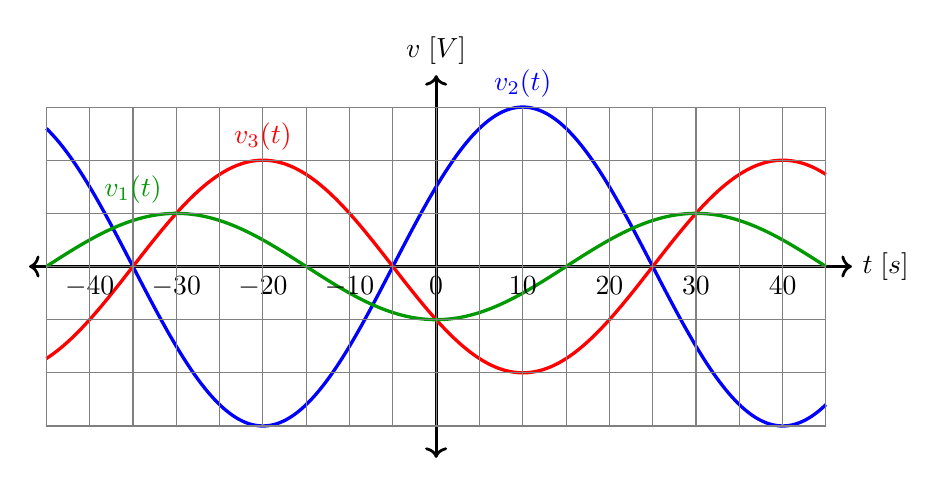
\begin{tikzpicture}[xscale=0.11, yscale=0.135]
    \draw[<->,line width=1pt] (-47,0) -- (48,0) node[right] {$t\hspace{1mm}[s]$};
    \draw[<->,line width=1pt] (0,-18) -- (0,18) node[above] {$v\hspace{1mm}[V]$};

%i2
    \draw[scale=1,domain=-45:45,variable=\x,blue,line width=1.2pt,samples=1000,opacity=1] 
    %plot({\x},{15*cos(((3.1415927/30)*\x-(3.1415927/2)) r)});
    plot({\x},{15*cos(((3.1415927/30)*\x-(1*3.1415927/3)) r)});
%i3
    \draw[scale=1,domain=-45:45,variable=\x,red,line width=1.2pt,samples=1000,opacity=1] 
    plot({\x},{10*cos(((3.1415927/30)*\x-(4*3.1415927/3)) r)});
%i1   
 \draw[scale=1,domain=-45:45,variable=\x,black!40!green,line width=1.2pt,samples=1000,opacity=1] 
    plot({\x},{5*cos(((3.1415927/30)*\x+(3*3.1415927/3)) r)});
      
      
    
    \foreach \i in {-40,-30,-20,-10,0,10,20,30,40} {
        \draw (\i,0) -- (\i,-0.05) node[below] {$\i$};
    }

%    \draw (0,15) -- (0.05,15) node[right] {$6$};
%    \draw (0,-15.15) -- (0.05,-15.15) node[right] {$-6$};
    
    \draw[step=5cm,color=gray, thin] (-45.01,-15.01) grid (45,15);
    
    \draw (10,15) node[blue,above] {$v_{2}(t)$};
    \draw (-20,10) node[red,above] {$v_{3}(t)$};
    \draw (-35,5) node[black!40!green,above] {$v_{1}(t)$};

    
  \end{tikzpicture}

\end{document}